\documentclass[11pt,a4paper]{article}
\usepackage[margin=2.5cm]{geometry}
\usepackage[T1]{fontenc}
\usepackage[utf8]{inputenc}

\usepackage{cite}
\usepackage{amsmath,amssymb,amsfonts}
\usepackage{algorithm}
\usepackage{algpseudocode}
\usepackage{graphicx}
\usepackage[section]{placeins}
\usepackage{tikz}
\usetikzlibrary{arrows.meta,calc}
\usepackage{booktabs}
\usepackage{multirow}
\usepackage{xcolor}
\usepackage{url}
\usepackage[hidelinks]{hyperref}
\usepackage{amsthm}

\theoremstyle{definition}
\newtheorem{definition}{Definition}
\newtheorem{assumption}{Assumption}
\theoremstyle{plain}
\newtheorem{lemma}{Lemma}
\newtheorem{proposition}{Proposition}
\newtheorem{theorem}{Theorem}
\newtheorem{corollary}{Corollary}
\theoremstyle{remark}
\newtheorem{remark}{Remark}

\newcommand{\N}{\mathbb{N}}
\newcommand{\R}{\mathbb{R}}
\newcommand{\Fac}{\mathbb{F}}
\newcommand{\Mon}{\mathfrak{M}}
\newcommand{\Gen}{\mathcal{T}}
\newcommand{\M}{\mathbf{M}}
\newcommand{\Rs}{\mathcal{R}}
\newcommand{\F}{\mathbf{F}}
\newcommand{\ND}{\operatorname{ND}}
\newcommand{\HV}{\operatorname{HV}}
\newcommand{\one}{\mathbb{1}}

% gerado automaticamente por MGGP_multiobjetivo.ipynb (custo ops, rho = 1) -- não editar à mão
\newcommand{\nSeeds}{30}
\newcommand{\tauSel}{0.05}
\newcommand{\EBSOHVid}{0.640}
\newcommand{\EBSOHVval}{0.640}
\newcommand{\EBSOCsel}{9}
\newcommand{\EBSOVALsel}{0.000}
\newcommand{\EBSORec}{100}
\newcommand{\EBSORecFront}{100}
\newcommand{\EBSOExtra}{1}
\newcommand{\EBSOTime}{0.9}
\newcommand{\EBLexHVid}{0.829}
\newcommand{\EBLexHVval}{0.827}
\newcommand{\EBLexCsel}{7}
\newcommand{\EBLexVALsel}{0.000}
\newcommand{\EBLexRec}{100}
\newcommand{\EBLexRecFront}{100}
\newcommand{\EBLexExtra}{0}
\newcommand{\EBLexTime}{0.9}
\newcommand{\EBGreenHVid}{0.896}
\newcommand{\EBGreenHVval}{0.893}
\newcommand{\EBGreenCsel}{7}
\newcommand{\EBGreenVALsel}{0.000}
\newcommand{\EBGreenRec}{100}
\newcommand{\EBGreenRecFront}{100}
\newcommand{\EBGreenExtra}{0}
\newcommand{\EBGreenTime}{1.9}
\newcommand{\EBCostRatioSO}{22}
\newcommand{\EBCostRatioLex}{0}
\newcommand{\ECSOHVid}{0.508}
\newcommand{\ECSOHVval}{0.505}
\newcommand{\ECSOCsel}{12}
\newcommand{\ECSOVALsel}{0.028}
\newcommand{\ECSORec}{0}
\newcommand{\ECSORecFront}{0}
\newcommand{\ECSOExtra}{5}
\newcommand{\ECSOTime}{1.1}
\newcommand{\ECLexHVid}{0.702}
\newcommand{\ECLexHVval}{0.699}
\newcommand{\ECLexCsel}{10}
\newcommand{\ECLexVALsel}{0.028}
\newcommand{\ECLexRec}{0}
\newcommand{\ECLexRecFront}{7}
\newcommand{\ECLexExtra}{4}
\newcommand{\ECLexTime}{1.2}
\newcommand{\ECGreenHVid}{0.879}
\newcommand{\ECGreenHVval}{0.874}
\newcommand{\ECGreenCsel}{7}
\newcommand{\ECGreenVALsel}{0.028}
\newcommand{\ECGreenRec}{0}
\newcommand{\ECGreenRecFront}{0}
\newcommand{\ECGreenExtra}{3}
\newcommand{\ECGreenTime}{2.2}
\newcommand{\ECCostRatioSO}{42}
\newcommand{\ECCostRatioLex}{30}
\newcommand{\EDSOHVid}{0.736}
\newcommand{\EDSOHVval}{0.000}
\newcommand{\EDSOCsel}{18.5}
\newcommand{\EDSOVALsel}{1.394}
\newcommand{\EDSORec}{0}
\newcommand{\EDSORecFront}{0}
\newcommand{\EDSOExtra}{7}
\newcommand{\EDSOTime}{1.9}
\newcommand{\EDLexHVid}{0.798}
\newcommand{\EDLexHVval}{0.000}
\newcommand{\EDLexCsel}{16}
\newcommand{\EDLexVALsel}{1.411}
\newcommand{\EDLexRec}{0}
\newcommand{\EDLexRecFront}{0}
\newcommand{\EDLexExtra}{6}
\newcommand{\EDLexTime}{2.0}
\newcommand{\EDGreenHVid}{0.954}
\newcommand{\EDGreenHVval}{0.893}
\newcommand{\EDGreenCsel}{16}
\newcommand{\EDGreenVALsel}{1.453}
\newcommand{\EDGreenRec}{0}
\newcommand{\EDGreenRecFront}{0}
\newcommand{\EDGreenExtra}{6}
\newcommand{\EDGreenTime}{3.2}
\newcommand{\EDCostRatioSO}{14}
\newcommand{\EDCostRatioLex}{0}
\newcommand{\costMulAdd}{11.4}
\newcommand{\rhoK}{11.39}
\newcommand{\rhoVal}{1}
\newcommand{\Ctrue}{7}
\newcommand{\Cfour}{9}
\newcommand{\EBCref}{25}
\newcommand{\ECCref}{25}
\newcommand{\EDCref}{72}
\newcommand{\EBLexSame}{30}
\newcommand{\EBGreenMaxU}{8}
\newcommand{\EBLbound}{50}
\newcommand{\EBSOHVdrops}{30}
\newcommand{\EBLexHVdrops}{30}
\newcommand{\EBGreenHVdrops}{0}
\newcommand{\ECLexSame}{30}
\newcommand{\ECGreenMaxU}{9}
\newcommand{\ECLbound}{50}
\newcommand{\ECSOHVdrops}{30}
\newcommand{\ECLexHVdrops}{30}
\newcommand{\ECGreenHVdrops}{0}
\newcommand{\EDLexSame}{30}
\newcommand{\EDGreenMaxU}{12}
\newcommand{\EDLbound}{260}
\newcommand{\EDSOHVdrops}{30}
\newcommand{\EDLexHVdrops}{30}
\newcommand{\EDGreenHVdrops}{0}
\newcommand{\ECRecTauSOApA}{0}
\newcommand{\ECRecTauSOApAB}{0}
\newcommand{\ECRecTauSOApAC}{0}
\newcommand{\ECRecTauSOApAF}{0}
\newcommand{\ECRecTauSOApB}{0}
\newcommand{\ECRecTauSOApC}{0}
\newcommand{\ECRecTauSOApF}{0}
\newcommand{\ECRecTauSOBpA}{0}
\newcommand{\ECRecTauLexApA}{0}
\newcommand{\ECRecTauLexApAB}{0}
\newcommand{\ECRecTauLexApAC}{0}
\newcommand{\ECRecTauLexApAF}{0}
\newcommand{\ECRecTauLexApB}{0}
\newcommand{\ECRecTauLexApC}{0}
\newcommand{\ECRecTauLexApF}{7}
\newcommand{\ECRecTauLexBpA}{7}
\newcommand{\ECRecTauGreenApA}{0}
\newcommand{\ECRecTauGreenApAB}{0}
\newcommand{\ECRecTauGreenApAC}{0}
\newcommand{\ECRecTauGreenApAF}{0}
\newcommand{\ECRecTauGreenApB}{0}
\newcommand{\ECRecTauGreenApC}{0}
\newcommand{\ECRecTauGreenApF}{0}
\newcommand{\ECRecTauGreenBpA}{0}
% comparação entre cenários de custo
\newcommand{\RhoEBOneGreenHVid}{0.896}
\newcommand{\RhoEBOneLexHVid}{0.829}
\newcommand{\RhoEBOneSOHVid}{0.640}
\newcommand{\RhoEBOneCostRed}{22}
\newcommand{\RhoEBOneGreenOps}{7}
\newcommand{\RhoEBOneGreenKar}{48.6}
\newcommand{\RhoEBKaraGreenHVid}{0.929}
\newcommand{\RhoEBKaraLexHVid}{0.884}
\newcommand{\RhoEBKaraSOHVid}{0.738}
\newcommand{\RhoEBKaraCostRed}{20}
\newcommand{\RhoEBKaraGreenOps}{7}
\newcommand{\RhoEBKaraGreenKar}{48.6}
\newcommand{\RhoEBSame}{100}
\newcommand{\RhoECOneGreenHVid}{0.879}
\newcommand{\RhoECOneLexHVid}{0.702}
\newcommand{\RhoECOneSOHVid}{0.508}
\newcommand{\RhoECOneCostRed}{42}
\newcommand{\RhoECOneGreenOps}{7}
\newcommand{\RhoECOneGreenKar}{48.6}
\newcommand{\RhoECKaraGreenHVid}{0.911}
\newcommand{\RhoECKaraLexHVid}{0.773}
\newcommand{\RhoECKaraSOHVid}{0.622}
\newcommand{\RhoECKaraCostRed}{43}
\newcommand{\RhoECKaraGreenOps}{7}
\newcommand{\RhoECKaraGreenKar}{48.6}
\newcommand{\RhoECSame}{93}
\newcommand{\RhoEDOneGreenHVid}{0.954}
\newcommand{\RhoEDOneLexHVid}{0.798}
\newcommand{\RhoEDOneSOHVid}{0.736}
\newcommand{\RhoEDOneCostRed}{14}
\newcommand{\RhoEDOneGreenOps}{16}
\newcommand{\RhoEDOneGreenKar}{109.5}
\newcommand{\RhoEDKaraGreenHVid}{0.962}
\newcommand{\RhoEDKaraLexHVid}{0.874}
\newcommand{\RhoEDKaraSOHVid}{0.819}
\newcommand{\RhoEDKaraCostRed}{14}
\newcommand{\RhoEDKaraGreenOps}{16}
\newcommand{\RhoEDKaraGreenKar}{109.5}
\newcommand{\RhoEDSame}{3}

% gerado automaticamente por MGGP_multiobjetivo.ipynb (custo karatsuba, rho = 11.3906) -- não editar à mão
\newcommand{\KaranSeeds}{30}
\newcommand{\KaratauSel}{0.05}
\newcommand{\KaraEBSOHVid}{0.738}
\newcommand{\KaraEBSOHVval}{0.738}
\newcommand{\KaraEBSOCsel}{61.0}
\newcommand{\KaraEBSOVALsel}{0.000}
\newcommand{\KaraEBSORec}{100}
\newcommand{\KaraEBSORecFront}{100}
\newcommand{\KaraEBSOExtra}{1}
\newcommand{\KaraEBSOTime}{0.8}
\newcommand{\KaraEBLexHVid}{0.884}
\newcommand{\KaraEBLexHVval}{0.883}
\newcommand{\KaraEBLexCsel}{48.6}
\newcommand{\KaraEBLexVALsel}{0.000}
\newcommand{\KaraEBLexRec}{100}
\newcommand{\KaraEBLexRecFront}{100}
\newcommand{\KaraEBLexExtra}{0}
\newcommand{\KaraEBLexTime}{0.7}
\newcommand{\KaraEBGreenHVid}{0.929}
\newcommand{\KaraEBGreenHVval}{0.927}
\newcommand{\KaraEBGreenCsel}{48.6}
\newcommand{\KaraEBGreenVALsel}{0.000}
\newcommand{\KaraEBGreenRec}{100}
\newcommand{\KaraEBGreenRecFront}{100}
\newcommand{\KaraEBGreenExtra}{0}
\newcommand{\KaraEBGreenTime}{1.6}
\newcommand{\KaraEBCostRatioSO}{20}
\newcommand{\KaraEBCostRatioLex}{0}
\newcommand{\KaraECSOHVid}{0.622}
\newcommand{\KaraECSOHVval}{0.618}
\newcommand{\KaraECSOCsel}{84.7}
\newcommand{\KaraECSOVALsel}{0.028}
\newcommand{\KaraECSORec}{0}
\newcommand{\KaraECSORecFront}{0}
\newcommand{\KaraECSOExtra}{5}
\newcommand{\KaraECSOTime}{0.9}
\newcommand{\KaraECLexHVid}{0.773}
\newcommand{\KaraECLexHVval}{0.768}
\newcommand{\KaraECLexCsel}{72.3}
\newcommand{\KaraECLexVALsel}{0.028}
\newcommand{\KaraECLexRec}{0}
\newcommand{\KaraECLexRecFront}{7}
\newcommand{\KaraECLexExtra}{4}
\newcommand{\KaraECLexTime}{0.8}
\newcommand{\KaraECGreenHVid}{0.911}
\newcommand{\KaraECGreenHVval}{0.906}
\newcommand{\KaraECGreenCsel}{48.6}
\newcommand{\KaraECGreenVALsel}{0.028}
\newcommand{\KaraECGreenRec}{0}
\newcommand{\KaraECGreenRecFront}{0}
\newcommand{\KaraECGreenExtra}{3}
\newcommand{\KaraECGreenTime}{1.8}
\newcommand{\KaraECCostRatioSO}{43}
\newcommand{\KaraECCostRatioLex}{33}
\newcommand{\KaraEDSOHVid}{0.819}
\newcommand{\KaraEDSOHVval}{0.000}
\newcommand{\KaraEDSOCsel}{127.6}
\newcommand{\KaraEDSOVALsel}{1.394}
\newcommand{\KaraEDSORec}{0}
\newcommand{\KaraEDSORecFront}{0}
\newcommand{\KaraEDSOExtra}{7}
\newcommand{\KaraEDSOTime}{1.5}
\newcommand{\KaraEDLexHVid}{0.874}
\newcommand{\KaraEDLexHVval}{0.000}
\newcommand{\KaraEDLexCsel}{109.5}
\newcommand{\KaraEDLexVALsel}{1.411}
\newcommand{\KaraEDLexRec}{0}
\newcommand{\KaraEDLexRecFront}{0}
\newcommand{\KaraEDLexExtra}{6}
\newcommand{\KaraEDLexTime}{1.3}
\newcommand{\KaraEDGreenHVid}{0.962}
\newcommand{\KaraEDGreenHVval}{0.904}
\newcommand{\KaraEDGreenCsel}{109.5}
\newcommand{\KaraEDGreenVALsel}{1.382}
\newcommand{\KaraEDGreenRec}{0}
\newcommand{\KaraEDGreenRecFront}{0}
\newcommand{\KaraEDGreenExtra}{6}
\newcommand{\KaraEDGreenTime}{2.5}
\newcommand{\KaraEDCostRatioSO}{14}
\newcommand{\KaraEDCostRatioLex}{0}
\newcommand{\KaracostMulAdd}{11.4}
\newcommand{\KararhoK}{11.39}
\newcommand{\KararhoVal}{11.39}
\newcommand{\KaraCtrue}{48.6}
\newcommand{\KaraCfour}{61.0}
\newcommand{\KaraEBCref}{232.8}
\newcommand{\KaraECCref}{232.8}
\newcommand{\KaraEDCref}{737.0}
\newcommand{\KaraEBLexSame}{30}
\newcommand{\KaraEBGreenMaxU}{8}
\newcommand{\KaraEBLbound}{50}
\newcommand{\KaraEBSOHVdrops}{30}
\newcommand{\KaraEBLexHVdrops}{30}
\newcommand{\KaraEBGreenHVdrops}{0}
\newcommand{\KaraECLexSame}{30}
\newcommand{\KaraECGreenMaxU}{9}
\newcommand{\KaraECLbound}{50}
\newcommand{\KaraECSOHVdrops}{30}
\newcommand{\KaraECLexHVdrops}{30}
\newcommand{\KaraECGreenHVdrops}{0}
\newcommand{\KaraEDLexSame}{30}
\newcommand{\KaraEDGreenMaxU}{12}
\newcommand{\KaraEDLbound}{260}
\newcommand{\KaraEDSOHVdrops}{30}
\newcommand{\KaraEDLexHVdrops}{30}
\newcommand{\KaraEDGreenHVdrops}{0}
\newcommand{\KaraECRecTauSOApA}{0}
\newcommand{\KaraECRecTauSOApAB}{0}
\newcommand{\KaraECRecTauSOApAC}{0}
\newcommand{\KaraECRecTauSOApAF}{0}
\newcommand{\KaraECRecTauSOApB}{0}
\newcommand{\KaraECRecTauSOApC}{0}
\newcommand{\KaraECRecTauSOApF}{0}
\newcommand{\KaraECRecTauSOBpA}{0}
\newcommand{\KaraECRecTauLexApA}{0}
\newcommand{\KaraECRecTauLexApAB}{0}
\newcommand{\KaraECRecTauLexApAC}{0}
\newcommand{\KaraECRecTauLexApAF}{0}
\newcommand{\KaraECRecTauLexApB}{0}
\newcommand{\KaraECRecTauLexApC}{0}
\newcommand{\KaraECRecTauLexApF}{7}
\newcommand{\KaraECRecTauLexBpA}{7}
\newcommand{\KaraECRecTauGreenApA}{0}
\newcommand{\KaraECRecTauGreenApAB}{0}
\newcommand{\KaraECRecTauGreenApAC}{0}
\newcommand{\KaraECRecTauGreenApAF}{0}
\newcommand{\KaraECRecTauGreenApB}{0}
\newcommand{\KaraECRecTauGreenApC}{0}
\newcommand{\KaraECRecTauGreenApF}{0}
\newcommand{\KaraECRecTauGreenBpA}{0}

\begin{document}
\title{Corrected Green MGGP Experiments: native}
\author{}\date{}\maketitle
\section*{Notas}
\begin{itemize}
\item \textbf{O que mudou no MGGP:} o Green usa seleção de Pareto (NSGA-II), considerando erro e custo juntos. O modo MO-lex prioriza o erro e usa o custo para desempatar.
\item \textbf{Correção comum:} no estudo novo, um avaliador externo corrige os atrasos de entrada e saída para todos os métodos. Mantém mínimos quadrados e os operadores; simulações que divergem são falhas, não zeros. O pacote original não foi editado.
\item \textbf{Complexidade:} contamos as operações do polinômio sem termos repetidos: $C_\rho=a+\rho b$, com $a$ adições e $b$ multiplicações, incluindo os coeficientes. Isto é custo aritmético, não energia medida.
\item \textbf{Dois pesos:} $\rho=1$ conta todas as operações igualmente; $\rho_K=729/64$ vem do modelo teórico em bits de Karatsuba. Os dois foram fixados antes das novas buscas e continuam na análise.
\item \textbf{Medições:} tempos de execução permitem estimar $t_\times/t_+$; powermetrics mede potência para calcular energia; CodeCarbon fornece apenas a intensidade de carbono para calcular CO$_2$e. Energia e CodeCarbon não definem $\rho$.
\item \textbf{Comparações novas:} além do protocolo original, todos os métodos receberam 4.510 avaliações por corrida. Também comparamos objetivos de número de termos e de nós, sem mudar a regra de escolha do modelo.
\item \textbf{Estado deste relatório:} identificação corrigida concluída; energia dos novos modelos ainda pendente. As medições antigas não entram neste relatório.
\end{itemize}

\section{Corrected evaluator and experimental protocol}
\noindent This export uses corrected delayed-factor evaluation for every method. Least squares retains one column per gene, including duplicates; simulation uses the actual maximum factor delay for initialisation and complete windows of that delay plus $K=20$. Divergence is a failure. The vendored package is unchanged; a shared external evaluator implements these corrections.

This diagnostic retains the native offspring counts (90 for the baselines, 100 for Green) and reuse of valid fitness. Actual evaluation counts are in the saved CSVs; this arm is not an equal-budget comparison.

NSGA-II supplies Pareto ranking and crowding~\cite{DPAM2002}; the underlying multigene package is attributed to its software source~\cite{mggpy}. Thirty seeds were run for each example and configuration under both weights. E1 is generated by
\begin{equation}y(k)=0.65y(k-1)+0.35u(k)+0.10u(k)y(k-1),\label{eq:tutorial}\end{equation}
with white Gaussian measurement noise added in E2; E3 uses the Bouc--Wen simulator. The reference point remains $(1,1)$ and the declared cost reference is unchanged. Reference sensitivity is exported separately~\cite{Ishibuchi2018}. Holm correction includes all tested metrics, examples and baselines within each arm and weight (30 tests for the native arm, 60 for the equal-call arm). Run times under concurrent workloads, if present, are diagnostic rather than execution benchmarks.
\begin{table}[t]
\centering
\caption{Examples and search settings; $C_\mathrm{ref}$ for $\rho=1$ (common: population 100, 50 generations, crossover 0.9, initial mutation 0.2; baseline elite retention 10\%, multiple-shooting horizon $K=20$, primitives \texttt{mul} and $q^{-j}$).}
\label{tab:setup}
\setlength{\tabcolsep}{4pt}
\begin{tabular}{lcccccc}
\toprule
Example & $N_\mathrm{id}$ & $N_\mathrm{val}$ & genes & height & $j_{\max}$ & $C_\mathrm{ref}$ \\
\midrule
E1 Tutorial (noise-free) & 210 & 90 & 5 & 2 & 2 & 25 \\
E2 Tutorial (noisy) & 210 & 90 & 5 & 2 & 2 & 25 \\
E3 Bouc--Wen hysteresis & 300 & 200 & 8 & 3 & 3 & 72 \\
\bottomrule
\end{tabular}
\end{table}

\section{Arithmetic complexity and declared weights}
For each duplicate-free polynomial, $C_\rho=a+\rho b$: $a$ counts additions and $b$ counts multiplications, including coefficients. This theoretical operation model is evaluated directly from the structure. Both fixed scenarios are analysed: $\rho=1$ counts operations equally; $\rho_K=729/64$ is the Green-Box bit-level weight associated with Karatsuba~\cite{NMN2023,KO1963}. Neither comes from measured power or CodeCarbon. The structural invariance and cost properties remain analytical results; population hashes and conditional hypervolume checks test the corresponding search statements empirically.

Timing calibration fits $t=t_0+t_+a+t_\times b$ and estimates $t_\times/t_+$ for the chosen execution implementation. Earlier Python timing measurements motivate an order-one primary weight; both weights were fixed before these corrected searches. The separate C microbenchmark is a diagnostic, not a calibration of CPython and not a reason to retune the objectives retrospectively. Powermetrics supplies power for energy integration; CodeCarbon supplies only grid carbon intensity. Corrected energy measurements remain pending.

\section{Results under both weights}
\begin{table*}[t]
\centering
\caption{Results over 30 independent runs with $\rho=1$: median [interquartile range]. HV: hypervolume of the delivered set (identification or free-run validation error); $C_\tau$, NRMSE$_\tau$: cost and free-run validation NRMSE of the model selected by the $\tau$-rule; Rec.$_\tau$, Rec.$_\mathcal{P}$: fraction of runs in which the selected model, or at least one model of the returned set, contains the three true regressors of \eqref{eq:tutorial}. $^{\ast}$/$^{\dagger}$: Green differs from SO/MO-lex (Mann--Whitney, Holm-adjusted $p<0.05$).}
\label{tab:results}
\footnotesize
\setlength{\tabcolsep}{2.5pt}
\resizebox{\textwidth}{!}{%
\begin{tabular}{llcccccc}
\toprule
Ex. & Method & HV$_\mathrm{id}$ & HV$_\mathrm{val}$ & $C_\tau$ & NRMSE$_\tau$ & Rec.$_\tau$ & Rec.$_\mathcal{P}$ \\
\midrule
\multirow{3}{*}{E1} & SO & 0.640 [0.560, 0.640] & 0.640 [0.560, 0.640] & 9 [9, 11] & 3e-16 [2e-16, 3e-16] & 1.00 & 1.00 \\
 & MO-lex & 0.829 [0.803, 0.829] & 0.827 [0.798, 0.827] & 7 [7, 7] & 3e-16 [3e-16, 3e-16] & 1.00 & 1.00 \\
 & \textbf{Green} & 0.896 [0.896, 0.896]$^{\ast}$$^{\dagger}$ & 0.893 [0.893, 0.893]$^{\ast}$$^{\dagger}$ & 7 [7, 7]$^{\ast}$ & 1e-15 [7e-16, 2e-15]$^{\ast}$$^{\dagger}$ & 1.00 & 1.00 \\
\midrule
\multirow{3}{*}{E2} & SO & 0.508 [0.508, 0.508] & 0.505 [0.505, 0.505] & 12 [12, 12] & 0.028 [0.028, 0.028] & 0.00 & 0.00 \\
 & MO-lex & 0.702 [0.661, 0.703] & 0.699 [0.656, 0.700] & 10 [9, 10] & 0.028 [0.028, 0.029] & 0.00 & 0.07 \\
 & \textbf{Green} & 0.879 [0.878, 0.881]$^{\ast}$$^{\dagger}$ & 0.874 [0.872, 0.876]$^{\ast}$$^{\dagger}$ & 7 [7, 7]$^{\ast}$$^{\dagger}$ & 0.028 [0.028, 0.028] & 0.00 & 0.00 \\
\midrule
\multirow{3}{*}{E3} & SO & 0.736 [0.729, 0.770] & 0.000 [0.000, 0.000] & 18.5 [16, 19] & 1.394 [1.301, 1.463] & -- & -- \\
 & MO-lex & 0.798 [0.797, 0.825] & 0.000 [0.000, 0.471] & 16 [16, 16] & 1.411 [1.340, 1.467] & -- & -- \\
 & \textbf{Green} & 0.954 [0.932, 0.956]$^{\ast}$$^{\dagger}$ & 0.893 [0.870, 0.893]$^{\ast}$$^{\dagger}$ & 16 [14.5, 16]$^{\ast}$ & 1.453 [1.353, 1.565] & -- & -- \\
\bottomrule
\end{tabular}}
\end{table*}

\begin{table}[t]
\centering
\caption{Regressors of the model selected by the $\tau$-rule in the representative run (median validation NRMSE of the selected model) and its free-run validation NRMSE.}
\label{tab:models}
\setlength{\tabcolsep}{3pt}
\footnotesize
\begin{tabular}{llp{8.5cm}rr}
\toprule
Ex. & Method & Regressors & $C$ & NRMSE \\
\midrule
E2 & SO & $u(k) y(k-2),\ u(k-1),\ y(k-2),\ y(k-2)^{2},\ y(k-5)$ & 12 & 0.028 \\
E2 & MO-lex & $u(k-1),\ u(k-1) y(k-2),\ y(k-5)$ & 7 & 0.028 \\
E2 & Green & $u(k-1),\ u(k-1) y(k-2),\ y(k-5)$ & 7 & 0.028 \\
\midrule
E3 & SO & $u(k-2) u(k-4) y(k-3),\ u(k-6),\ u(k-7),\ u(k-8),\ y(k-1),\ y(k-2),\ y(k-7),\ y(k-8)$ & 18 & 1.413 \\
E3 & MO-lex & $u(k-3) u(k-4) y(k-2),\ u(k-6),\ u(k-7),\ u(k-8),\ y(k-1),\ y(k-2),\ y(k-8)$ & 16 & 1.418 \\
E3 & Green & $u(k),\ u(k-1),\ u(k-2),\ u(k-6),\ y(k-1),\ y(k-7),\ y(k-8)$ & 14 & 1.457 \\
\bottomrule
\end{tabular}
\end{table}

\begin{table}[t]
\centering
\caption{Empirical verification of Theorems~2 and~3 over 30 seeds. Lexicographic reduction: seeds in which SO and MO-lex produce identical populations in all generations; diverging seeds in which the divergence is preceded by an error tie between individuals of different cost, and in which the populations involved contain at least two individuals with $J_E=\infty$; median generation of the first divergence. Non-deterioration: largest $|U_t^1|$ over all runs and generations, bound $L(G,h)$ of $L(G,h)$ and population size $\mu$; runs with at least one decrease of the population-front hypervolume.}
\label{tab:checks}
\small
\setlength{\tabcolsep}{4pt}
\begin{tabular}{lcccccccccc}
\toprule
 & \multicolumn{4}{c}{Lexicographic reduction} & \multicolumn{3}{c}{Capacity} & \multicolumn{3}{c}{Runs with HV decrease} \\
\cmidrule(lr){2-5}\cmidrule(lr){6-8}\cmidrule(lr){9-11}
Ex. & identical & tie & $J_E{=}\infty$ & first div. & $\max|U_t^1|$ & $L(G,h)$ & $\mu$ & SO & MO-lex & Green \\
\midrule
E1 & 30/30 & 0/0 & 0/0 & -- & 8 & 50 & 100 & 30 & 30 & 0 \\
E2 & 30/30 & 0/0 & 0/0 & -- & 9 & 50 & 100 & 30 & 30 & 0 \\
E3 & 30/30 & 0/0 & 0/0 & -- & 12 & 260 & 100 & 30 & 30 & 0 \\
\bottomrule
\end{tabular}
\end{table}

\begin{table}[t]
\centering
\caption{Effect of the multiplication weight $\rho$ over 30 runs (medians). HV: identification hypervolume; $\Delta C_\tau$: reduction of the median selected cost of Green MGGP relative to SO, with the cost of the same scenario; $a{+}b$ and $C_{\rho_K}$: operation count and Karatsuba-weighted cost of the selected Green model; same: fraction of seeds in which Green MGGP selects the same structure under both weights.}
\label{tab:rho}
\setlength{\tabcolsep}{3.5pt}
\small
\begin{tabular}{llccccccc}
\toprule
 & & \multicolumn{3}{c}{HV$_\mathrm{id}$} & & \multicolumn{2}{c}{Green $\mathcal M_\tau$} & \\
\cmidrule(lr){3-5}\cmidrule(lr){7-8}
Ex. & weight & SO & MO-lex & Green & $\Delta C_\tau$ & $a{+}b$ & $C_{\rho_K}$ & same \\
\midrule
E1 & $\rho=1$ & 0.640 & 0.829 & 0.896 & 22\% & 7 & 48.6 & 100\% \\
 & $\rho_K$ & 0.738 & 0.884 & 0.929 & 20\% & 7 & 48.6 &  \\
\midrule
E2 & $\rho=1$ & 0.508 & 0.702 & 0.879 & 42\% & 7 & 48.6 & 93\% \\
 & $\rho_K$ & 0.622 & 0.773 & 0.911 & 43\% & 7 & 48.6 &  \\
\midrule
E3 & $\rho=1$ & 0.736 & 0.798 & 0.954 & 14\% & 16 & 109.5 & 3\% \\
 & $\rho_K$ & 0.819 & 0.874 & 0.962 & 14\% & 16 & 109.5 &  \\
\bottomrule
\end{tabular}
\end{table}

\begin{figure}[p]\centering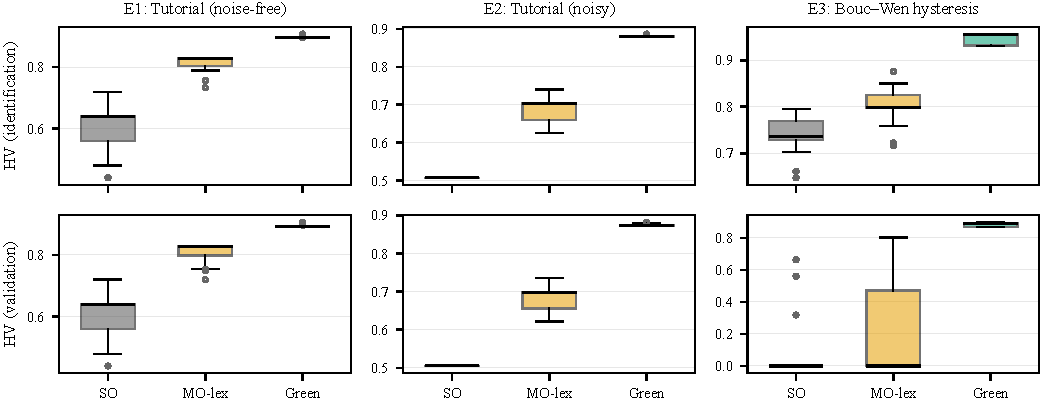
\includegraphics[width=\textwidth]{figures/fig_hv.pdf}\caption{Corrected results: hv.}\end{figure}
\begin{figure}[p]\centering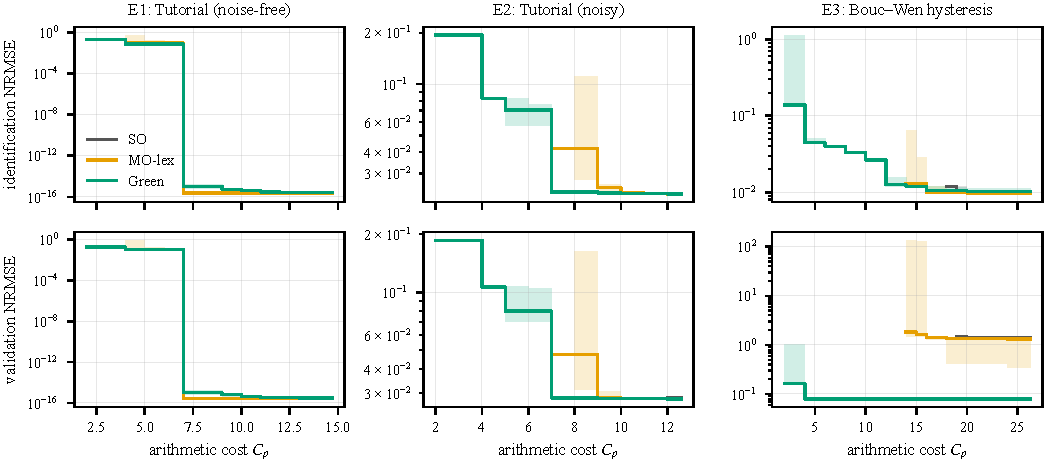
\includegraphics[width=\textwidth]{figures/fig_attainment.pdf}\caption{Corrected results: attainment.}\end{figure}
\begin{figure}[p]\centering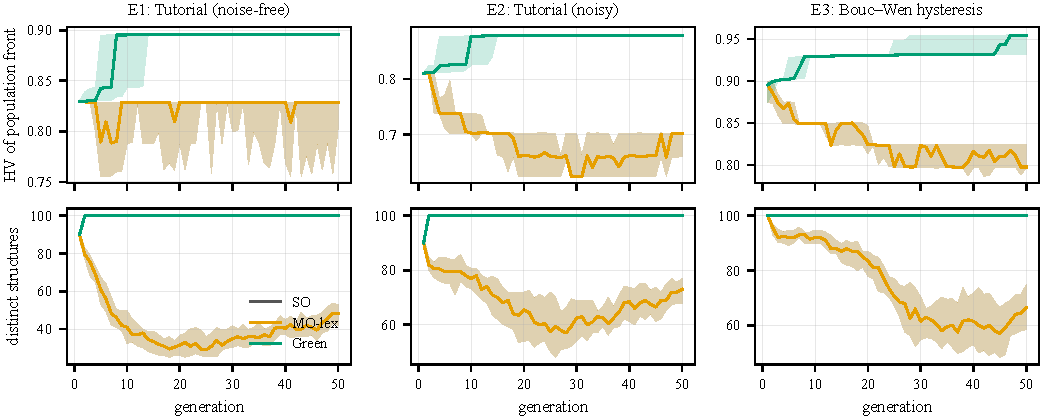
\includegraphics[width=\textwidth]{figures/fig_convergence.pdf}\caption{Corrected results: convergence.}\end{figure}
\begin{figure}[p]\centering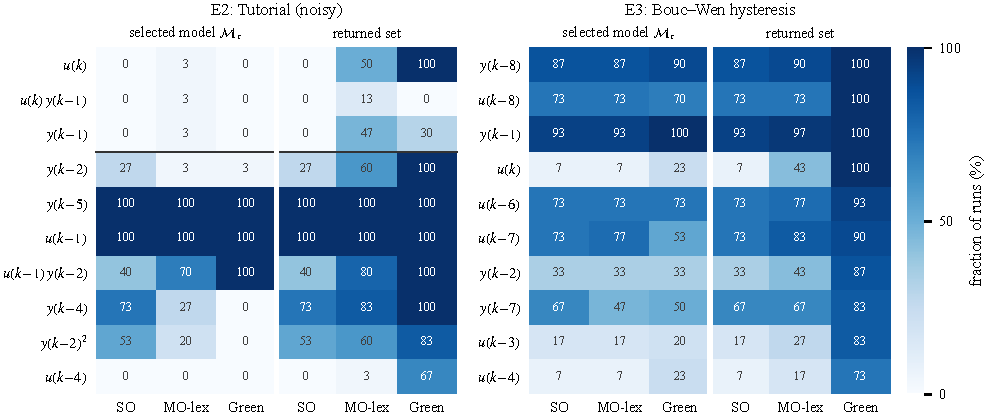
\includegraphics[width=\textwidth]{figures/fig_regressors.pdf}\caption{Corrected results: regressors.}\end{figure}
\begin{figure}[p]\centering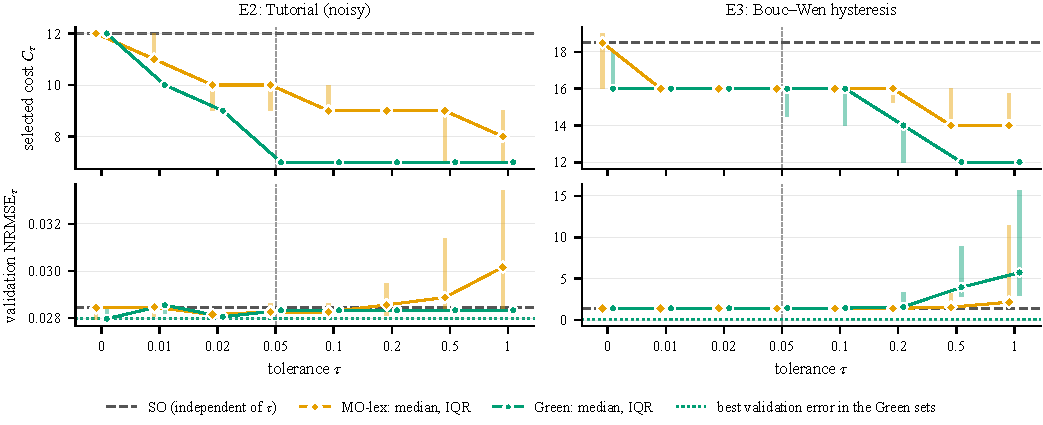
\includegraphics[width=\textwidth]{figures/fig_tau.pdf}\caption{Corrected results: tau.}\end{figure}
\begin{figure}[p]\centering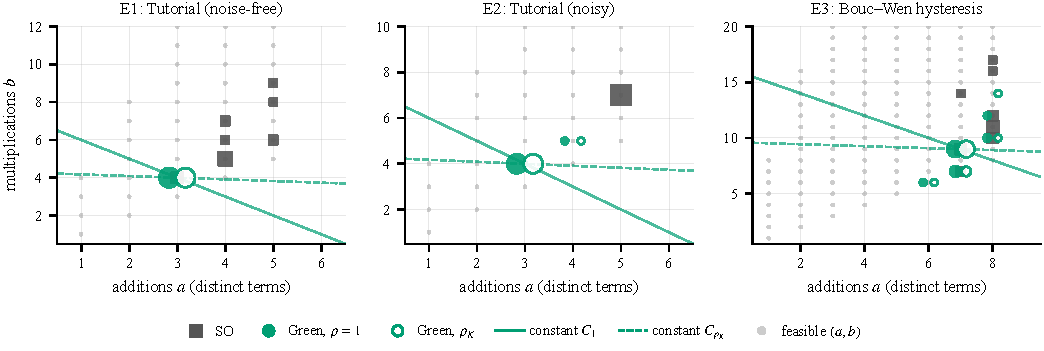
\includegraphics[width=\textwidth]{figures/fig_ab.pdf}\caption{Corrected results: ab.}\end{figure}
\begin{figure}[p]\centering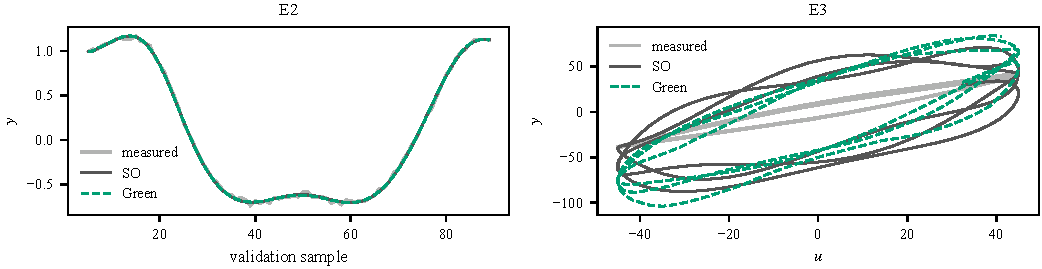
\includegraphics[width=\textwidth]{figures/fig_freerun.pdf}\caption{Corrected results: freerun.}\end{figure}
\clearpage
\noindent Energy and carbon measurements for these selected models are pending. Historical energy values are not included. The node and term ablations and their statistics are in the parent study report and CSVs.
\bibliographystyle{unsrt}\bibliography{refs}
\end{document}
